\subsubsection {Optimización cúmulos de partículas (PSO)}
La optimización mediante cúmulos de partículas es una heurística de la inteligencia colectiva desarrollada por Kennedy y Eberhart en 1995 según \cite{[KENNEDY]},  la cual se utiliza para resolver problemas de optimización colectiva, denominada PSO por sus siglas en inglés (Particle Swarm Optimization).\\
\hspace*{1cm}De acuerdo con \cite{[FLORES]} PSO tiene como motivación básica del comportamiento de algunos animales como los bancos de peces, donde se establecen relaciones sociales entre los individuos del grupo,  de acuerdo a las características de cada individuo surge un líder que es reconocido por los demás individuos del grupo. El líder del grupo tiene características que le permiten mantener el control sobre el grupo y guiarlos, (como se puede observar en la figura \ref{fig:natPSO}) que gracias a esto, los bancos de peces y las parvadas de aves se mueven de manera organizada sin estrellarse los unos a los otros.\\

   \begin{figure}[hbtp]
        \centering
            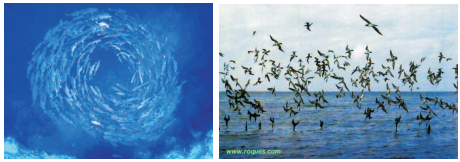
\includegraphics[width=1\textwidth]{MarcoTeorico/Imagenes/natPSO.png}
            \caption{Ejemplos del PSO en la naturaleza.}                       
            \label{fig:natPSO}
    \end{figure} 
    
\hspace*{1cm}Los individuos de menor jerarquía deben confiar en la capacidad del líder para dirigirlos, sin embargo dentro del grupo surge un individuo con mejores capacidades que el actual, sustituyéndolo en el mando del grupo. El algoritmo se basa en los siguientes principios:

\begin{itemize}
\item \textbf{Movimiento: }La partícula se desplaza hacia donde le indica su vector de velocidad, calculado cada iteración.
\item \textbf{Inercia: }Tendencia a moverse en la misma dirección que se movió la última vez.
\item \textbf{Memoria individual: }Tendencia a moverse hacia la mejor solución que ha encontrado hasta ahora.
\item \textbf{Memoria colectiva: }Tendencia a moverse hacia la mejor solución que ha encontrado hasta ahora todo el enjambre.
\end{itemize}


El código \ref{lst:PseudocodigoPSO} representa una demostración del PSO:\\

\begin{lstlisting}[language=C++, caption=Pseudocódigo PSO, label=lst:PseudocodigoPSO]
/* Algoritmo de PSO */
Inicio
  Crear un cumulo inicial de particulas de manera aleatoria
  Evaluar cada particula
  for(i=0; i< MAX_GEN;i++){
   Seleccionar al lider del cumulo con base en la evaluacion de cada particula.
   Aplica funcion de vuelo a todas las particulas del cumulo.
   Actualizar la memoria de cada particula.
  }
Fin;

\end{lstlisting}